\documentclass[10pt]{article}
\usepackage[utf8]{inputenc}
\usepackage[spanish]{babel}
\usepackage[usenames,dvipsnames,svgnames,table]{xcolor}
\usepackage{multirow}
\usepackage{diagbox}
\usepackage{booktabs}
\usepackage{anysize} 
\usepackage{hyperref}
\usepackage{helvet}
\renewcommand\refname{Referencias}
\marginsize{2cm}{2cm}{2.0cm}{2cm}
\usepackage{enumitem}
\usepackage{setspace}
\usepackage{scrextend}
\usepackage{amssymb}
\usepackage{mathtools}
\addtokomafont{labelinglabel}{\sffamily}

%% Graphics
\usepackage{graphicx}
\usepackage{color}
\usepackage{gensymb}
\usepackage{multirow}
\usepackage{caption}
\usepackage{float}
\graphicspath{{img/}}
\setlength{\parindent}{0cm}


\hypersetup{
	colorlinks=true,
	linkcolor=blue,
	filecolor=magenta,
	urlcolor=cyan,
	citecolor=blue
}




\begin{document}
	\title{Fundamentos de Bases de Datos \\
		Proyecto Final\\ Empresas inmobiliarias
	} 
	\author{Díaz Gómez Silvia \\
		Eugenio Aceves Narciso Isaac \\
		Quiroz Castañeda Edgar}
	\date{08 de Junio del 2019}
	\maketitle
	
	Se nos pide diseñar una base de datos para poder almacenar toda la información de  las inmobiliarias han proporcionado. Como el almacenamiento de la información debe estar en una base de datos relacional el diseño consta de tres partes, la primera parte corresponde al modelo Entidad-Relación, la segunda parte a la traducción del modelo entidad relación al modelo relacional y finalmente la normalización que nos permite quitar redundancia en las tablas generadas. 
	
	\section{Diagrama E/R del caso de uso}
	
	El siguiente diagrama esta basado de acuerdo a las especificaciones en el caso de uso.
	
	\begin{center}
		\begin{figure}[H]
			\centering
			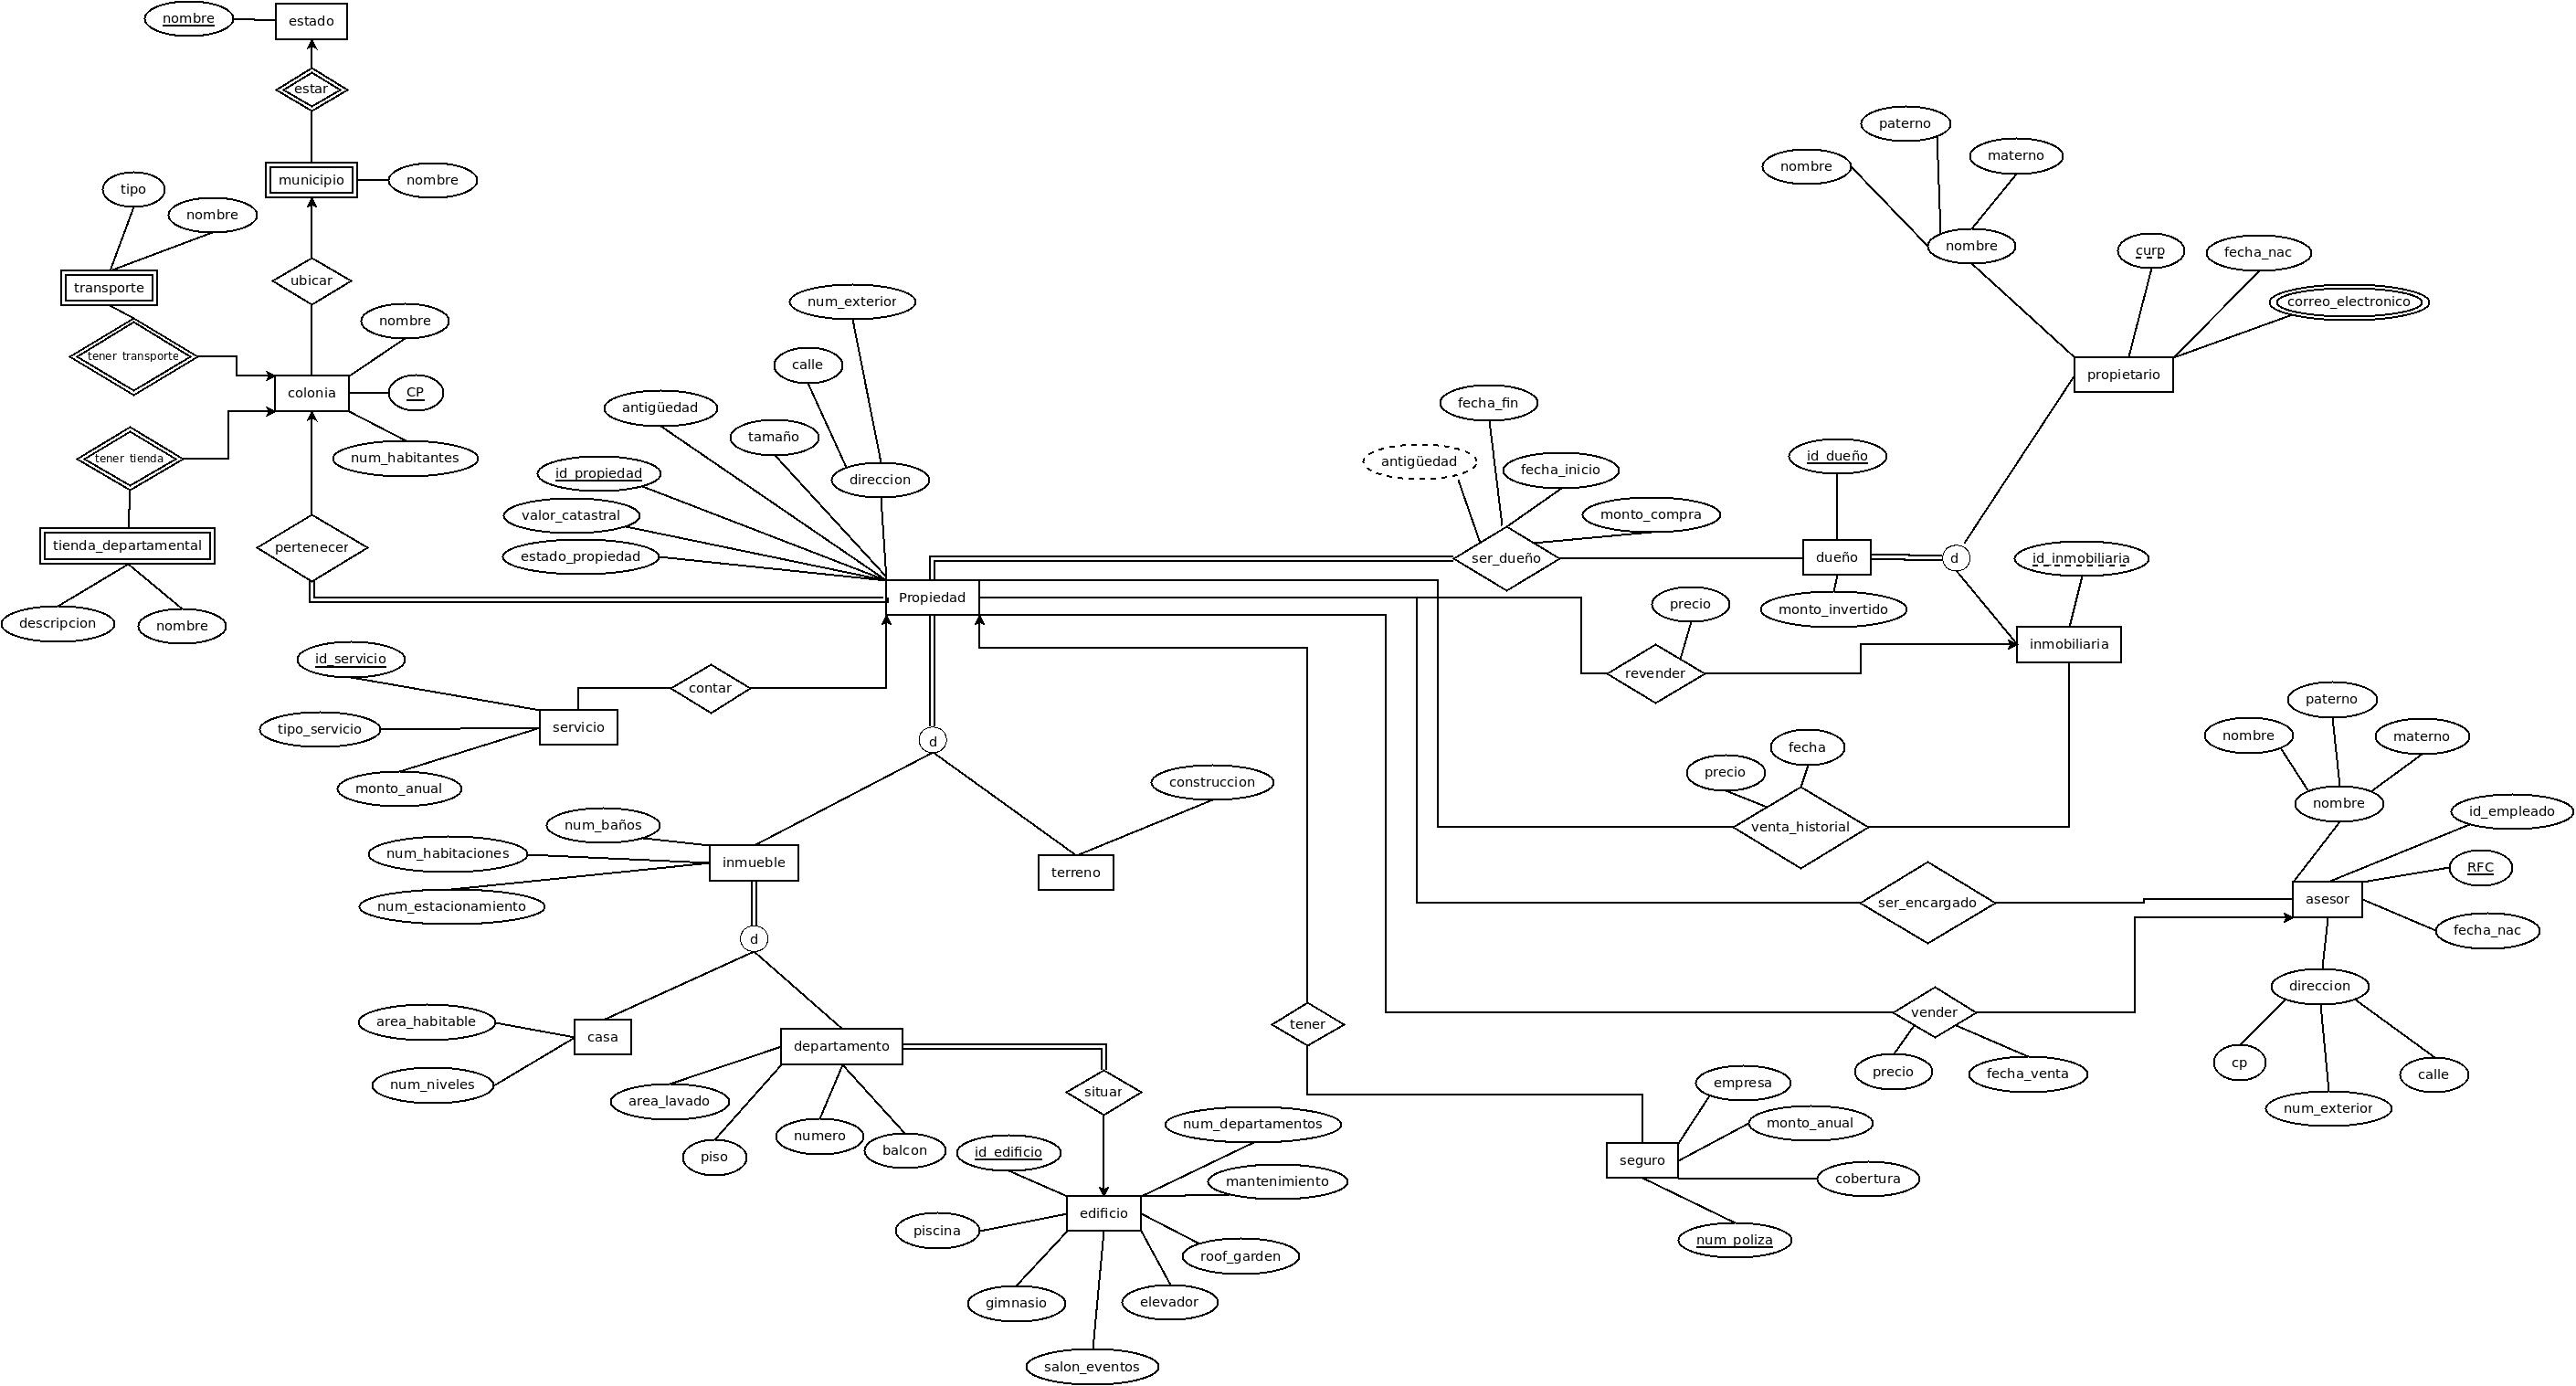
\includegraphics[width=1 \textwidth]{modeloER.jpeg}
			\caption{Diagrama E-R para las empresas inmobiliarias.}
			\label{ER}
		\end{figure}
	\end{center}
    \section{Modelo Relacional}
    
    \begin{center}
    	\begin{figure}[H]
    		\centering
    		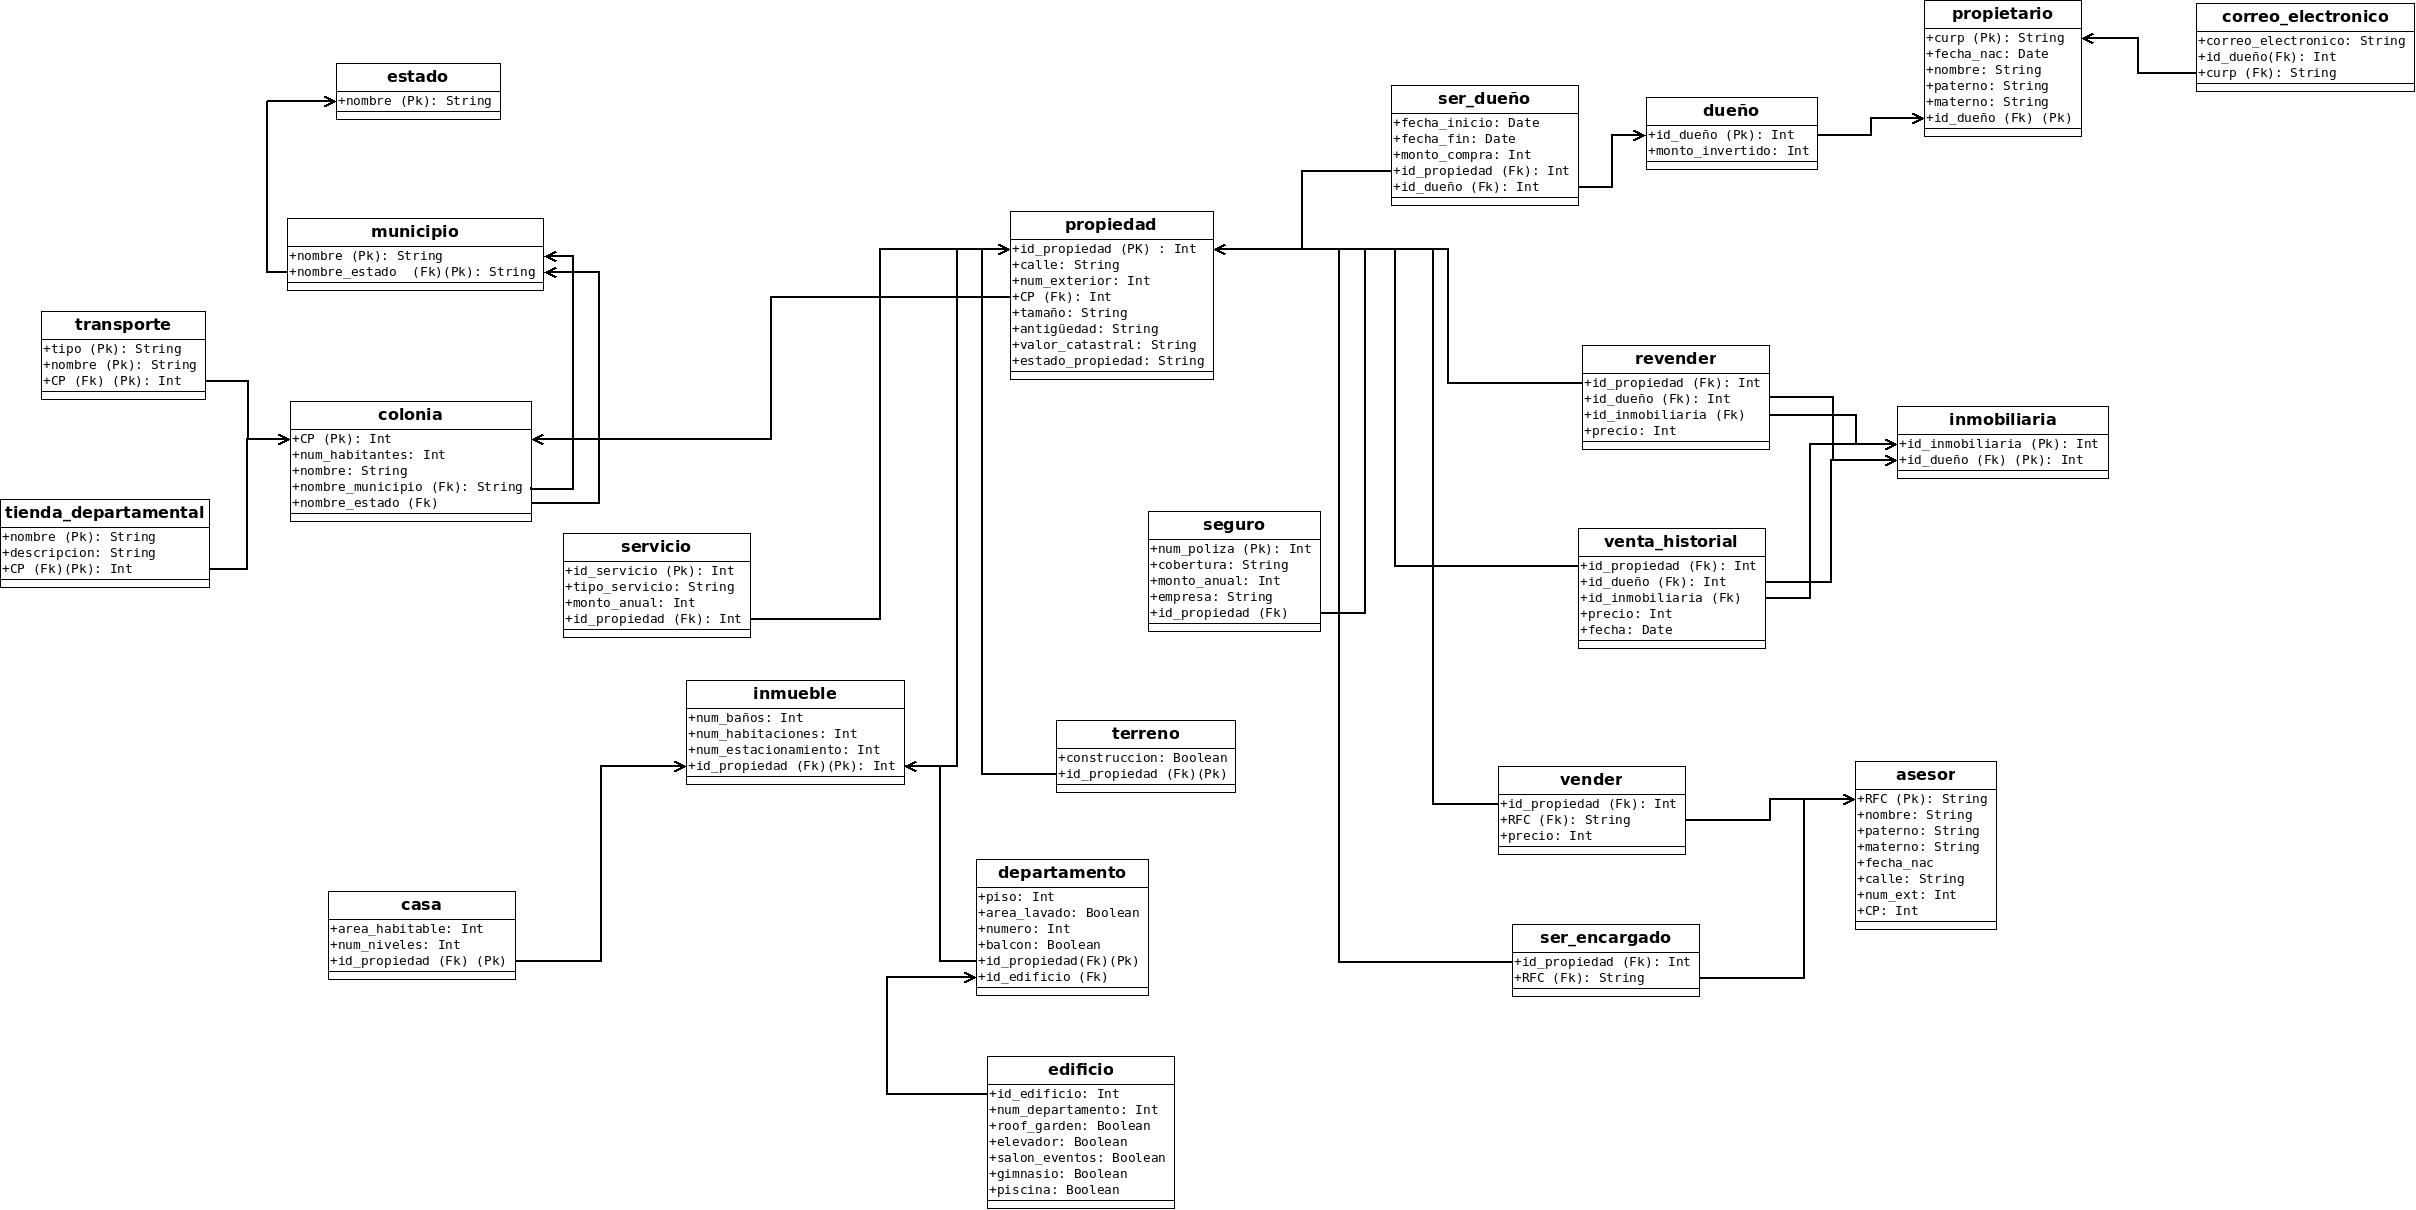
\includegraphics[width=1 \textwidth]{modeloRelacional.jpeg}
    		\caption{Traducción del diagrama del la figura \ref{ER} al modelo Relacional.}
    		\label{MR}
    	\end{figure}
    \end{center}

    \section{Normalización}
    
    Aquí se enlistan las relaciones que contenian dependencias funcionales triviales por lo tanto no fue necesario normalizarlas. 
    Todas las relaciones con únicamente dos atributos ya está normalizadas, pues las
    únicas dependencias funcionales que pueden haber son las triviales o las inducidas
    por llaves (un atributo determina al otro), y ninguna de estas es violación a la forma normal de BCNF.
    \begin{itemize}
    	\item Inmueble
    	\item Casa
    	\item Terreno
    	\item Departamento
    	\item Edificio
    	\item Ser dueño
    	\item Dueño
    	\item Correo 
    	\item Venta historial
    	\item Revender
    	\item Inmobiliaria
    	\item Vender
    	\item Ser encargado
    \end{itemize}
    
    En seguida se encuentran las relaciones que contienen dependencias no triviales o redundantes. Normalizamos de acuerdo a BCNF.
    
    \begin{enumerate}
    	\item \textbf{Colonia}
    	
    	La relación colonia es:
    	\[\overbrace{{\textbf{Colonia}}}^{\textbf{$R_{C}$}} 
    	(
    	\overbrace{CP}^{A}, \overbrace{num\_habitantes}^{B},
    	\overbrace{nombre}^{C}, \overbrace{nombre\_municipio}^{D}, \overbrace{nombre\_estado}^{E}
    	)
    	= 
    	\textbf{$R_C$}(A,B,C,D,E)
    	\]
    	
    	Y las dependencias funcionales encontratas en esta relación  y no triviales son:\\
    	\[\mathcal{F} = \{A \rightarrow CDE\}\]
    	
    	Lo siguiente sera determinar una llave para la relacion $R_C$ calculando la cerradura de la parte que se encuentran a la izquierda de las dependencias funcionales. La llave nos permitirá conocer si existen violaciones a la forma normal de BC.\\
    	
    	$\{\textcolor{RoyalBlue}{A}\}+= \{\textcolor{RoyalBlue}{A}CDE\}$\\
    	
    	El atributo $A$ casi alcanza a la mayoria de todos los atributos excepto a $B$, así que una llave para $R_C$ puede ser \textbf{AB}, ninguna de las dependecias funcionales cumple que la llave se encuentre a la izquierda de las dependencias funcionales por lo tanto son violaciones a BCNF.\\
    	\begin{itemize}
    		\item Para $A \rightarrow CDE$\\
    		Dividimos en dos relaciones la relacion original de acuerdo a los atributos de esta dependencia funcional, para la primera relación queda como:\\
    		
    		$\textbf{T}(A,C,D,E)$ con $A \rightarrow CDE$\\
    		
    		y para la suguiente relación se toman los atributos del lado izquierdo y los atributos restantes.\\
    		
    		$\textbf{S}(A,B)$ con $AB \rightarrow AB$\\ 
    		
    		No se tiene ninguna perdida de dependencias y observamos que en la relación
    		$\textbf{S}$ la dependencia que tiene es trivial por lo tanto no puede ser violación, entonces esta relación ya esta en forma normal de BCNF. \\
    		Para $\textbf{T}$  necesitamos encontrar una llave\\
    		$\{\textcolor{RoyalBlue}{A}\}+= \{\textcolor{RoyalBlue}{A}CDE\}$ la llave para $\textbf{T}$ es $A$, verificamos que esta este en todas las dependecias funcionales de la relación y como esta la cumple por lo tanto no existen violaciones, entonces la relación esta en forma normal de BCNF.\\
    	\end{itemize}
    
    Así que la normalización de la relación $R_C$ queda como:\\
    
    $\textbf{T}(A,C,D,E)$ con $A \rightarrow CDE$\\   
    $\textbf{S}(A,B)$ con $AB \rightarrow AB$\\
    
    
    \item \textbf{Propiertario}
    
    La relación propietario es:
    \[\overbrace{{\textbf{Propietario}}}^{\textbf{$R_{P}$}} 
    (
    \overbrace{curp}^{A}, \overbrace{fecha\_nac}^{B}, \overbrace{nombre}^{C}, \overbrace{paterno}^{D}, \overbrace{materno}^{E}, \overbrace{id\_dueno}^{F}
    )
    = 
    \textbf{$R_P$}(A,B,C,D,E,F)
    \]
    
    Y las dependencias funcionales encontratas en esta relación  y no triviales son:\\
    \[\mathcal{F} = \{A \rightarrow BCDE\}\]
    
    Buscamos una llave para la relacion $R_P$ calculando la cerradura de la parte que se encuentran a la izquierda de las dependencias funcionales. La llave nos permitirá conocer si existen violaciones a la forma normal de BC.\\
    
    $\{\textcolor{RoyalBlue}{A}\}+= \{\textcolor{RoyalBlue}{A}BCDE\}$\\
    
    El atributo $A$ casi alcanza a la mayoria de todos los atributos excepto a $F$, así que una llave para $R_C$ puede ser \textbf{AF}, ninguna de las dependecias funcionales cumple que la llave se encuentre a la izquierda de las dependencias funcionales por lo tanto son violaciones a BCNF.\\
    \begin{itemize}
    	\item Para $A \rightarrow BCDE$\\
    	Dividimos en dos relaciones la relacion original de acuerdo a los atributos de esta dependencia funcional, para la primera relación queda como:\\
    	
    	$\textbf{T}(A,B,C,D,E)$ con $A \rightarrow BCDE$\\
    	
    	y para la suguiente relación se toman los atributos del lado izquierdo y los atributos restantes.\\
    	
    	$\textbf{S}(A,F)$ con $AF \rightarrow AF$\\ 
    	
    	No se tiene ninguna perdida de dependencias y observamos que en la relación
    	$\textbf{S}$ la dependencia que tiene es trivial por lo tanto no puede ser violación, entonces esta relación ya esta en forma normal de BCNF. \\
    	Para $\textbf{T}$  necesitamos encontrar una llave\\
    	$\{\textcolor{RoyalBlue}{A}\}+= \{\textcolor{RoyalBlue}{A}BCDE\}$ la llave para $\textbf{T}$ es $A$, verificamos que esta este en todas las dependecias funcionales de la relación y como esta la cumple por lo tanto no existen violaciones, entonces la relación esta en forma normal de BCNF.\\
    \end{itemize}
    Así que la normalización de la relación $R_P$ queda como:\\
    
    	$\textbf{T}(A,B,C,D,E)$ con $A \rightarrow BCDE$\\   
    $\textbf{S}(A,F)$ con $AF \rightarrow AF$\\
   
   
   
   \item \textbf{Asesor}
   
   La relación asesor es:
   \[\overbrace{{\textbf{Asesor}}}^{\textbf{$R_{A}$}} 
   (
   \overbrace{RCF}^{A},
   \overbrace{nombre}^{B}, \overbrace{paterno}^{C}, \overbrace{materno}^{D}, \overbrace{fecha_nac}^{E}, \overbrace{calle}^{F}, \overbrace{num\_ext}^{G}, \overbrace{CP}^{H}
   )
   = 
   \textbf{$R_A$}(A,B,C,D,E,F,G,H)
   \]
   
   Y las dependencias funcionales encontratas en esta relación  y no triviales son:\\
   \[\mathcal{F} = \{A \rightarrow BCDE\}\]
   
   Buscamos una llave para la relacion $R_A$ calculando la cerradura de la parte que se encuentran a la izquierda de las dependencias funcionales. La llave nos permitirá conocer si existen violaciones a la forma normal de BC.\\
   
   $\{\textcolor{RoyalBlue}{A}\}+= \{\textcolor{RoyalBlue}{A}BCDE\}$\\
   
  Una llave para $R_A$ puede ser \textbf{AFGH}, ninguna de las dependecias funcionales cumple que la llave se encuentre a la izquierda de las dependencias funcionales por lo tanto son violaciones a BCNF.\\
   \begin{itemize}
   	\item Para $A \rightarrow BCDE$\\
   	Dividimos en dos relaciones la relacion original de acuerdo a los atributos de esta dependencia funcional, para la primera relación queda como:\\
   	
   	$\textbf{T}(A,B,C,D,E)$ con $A \rightarrow BCDE$\\
   	
   	y para la suguiente relación se toman los atributos del lado izquierdo y los atributos restantes.\\
   	
   	$\textbf{S}(A,F,G,H)$ con $AFGH \rightarrow AFGH$\\ 
   	
   	No se tiene ninguna perdida de dependencias y observamos que en la relación
   	$\textbf{S}$ la dependencia que tiene es trivial por lo tanto no puede ser violación, entonces esta relación ya esta en forma normal de BCNF. \\
   	Para $\textbf{T}$  necesitamos encontrar una llave\\
   	$\{\textcolor{RoyalBlue}{A}\}+= \{\textcolor{RoyalBlue}{A}BCDE\}$ la llave para $\textbf{T}$ es $A$, verificamos que esta este en todas las dependecias funcionales de la relación y como esta la cumple por lo tanto no existen violaciones, entonces la relación esta en forma normal de BCNF.\\
   \end{itemize}
   
    Así que la normalización de la relación $R_A$ queda como:\\
    
     	$\textbf{T}(A,B,C,D,E)$ con $A \rightarrow BCDE$\\   
    $\textbf{S}(A,F,G,H)$ con $AFGH \rightarrow AFGH$\\ 
    
    
    	
    	 
    	\item \textbf{Seguro}
    	
    	La relación seguro es:
    	\[\overbrace{{\textbf{Seguro}}}^{\textbf{$R_{S}$}} 
    	(
    	\overbrace{num\_poliza}^{A}, \overbrace{cobertura}^{B},
    	\overbrace{empresa}^{C}, \overbrace{monto\_anual}^{D}, \overbrace{id\_propiedad}^{E}
    	)
    	= 
    	\textbf{$R_S$}(A,B,C,D,E)
    	\]
    	
    	Y las dependencias funcionales encontratas en esta relación  y no triviales son:\\
    	\[\mathcal{F} = \{BCE \rightarrow D\}\]
    	
    	Lo siguiente sera determinar una llave para la relacion $R_S$ calculando la cerradura de la parte que se encuentran a la izquierda de las dependencias funcionales. La llave nos permitirá conocer si existen violaciones a la forma normal de BC.\\
    	
    	$\{\textcolor{RoyalBlue}{BCE}\}+= \{\textcolor{RoyalBlue}{BCE}D\}$\\
    	
    	Una llave para $R_S$ puede ser \textbf{BCEA}, ninguna de las dependecias funcionales cumple que la llave se encuentre a la izquierda de las dependencias funcionales por lo tanto son violaciones a BCNF.\\
    	\begin{itemize}
    		\item Para $BCE \rightarrow D$\\
    		Dividimos en dos relaciones la relacion original de acuerdo a los atributos de esta dependencia funcional, para la primera relación queda como:\\
    		
    		$\textbf{T}(B,C,E,D)$ con $BCE \rightarrow D$\\
    		
    		y para la suguiente relación se toman los atributos del lado izquierdo y los atributos restantes.\\
    		
    		$\textbf{S}(B,C,E,A)$ con $BCEA \rightarrow BCEA$\\ 
    		
    		No se tiene ninguna perdida de dependencias y observamos que en la relación
    		$\textbf{S}$ la dependencia que tiene es trivial por lo tanto no puede ser violación, entonces esta relación ya esta en forma normal de BCNF. \\
    		Para $\textbf{T}$  necesitamos encontrar una llave\\
    		$\{\textcolor{RoyalBlue}{BCE}\}+= \{\textcolor{RoyalBlue}{BCE}D\}$ la llave para $\textbf{T}$ es $BCE$, verificamos que esta este en todas las dependecias funcionales de la relación y como esta la cumple por lo tanto no existen violaciones, entonces la relación esta en forma normal de BCNF.\\
    	\end{itemize}
    	Así que la normalización de la relación $R_S$ queda como:\\
    	$\textbf{T}(B,C,E,D)$ con $BCE \rightarrow D$\\
    	$\textbf{S}(B,C,E,A)$ con $BCEA \rightarrow BCEA$\\ 
    	
    	\item \textbf{Propiedad}
    	
    	La relación propiedad es:
    	\begin{align*}
    	\overbrace{{\textbf{Propiedad}}}^{\textbf{$R_{P}$}} &
    	(
    	\overbrace{id\_propiedad}^{A}, \overbrace{calle}^{B},
    	\overbrace{num\_exterior}^{C}, \overbrace{CP}^{D}, \overbrace{tamano}^{E}, \overbrace{fecha_construccion}^{F}, \overbrace{valor\_catastral}^{G}, \overbrace{estado\_propiedad}^{H}
    	)\\
      &	= 
    	\textbf{$R_P$}(A,B,C,D,E,F,G,H)
    	\end{align*}
    	
    	Y las dependencias funcionales encontratas en esta relación  y no triviales son:\\
    	\[\mathcal{F} = \{DEFH \rightarrow G\}\]
    	
    	Lo siguiente sera determinar una llave para la relacion $R_P$ calculando la cerradura de la parte que se encuentran a la izquierda de las dependencias funcionales. La llave nos permitirá conocer si existen violaciones a la forma normal de BC.\\
    	
    	$\{\textcolor{RoyalBlue}{DEFH}\}+= \{\textcolor{RoyalBlue}{DEFH}G\}$\\
    	
    	Una llave para $R_P$ puede ser \textbf{DEFHABC}, ninguna de las dependecias funcionales cumple que la llave se encuentre a la izquierda de las dependencias funcionales por lo tanto son violaciones a BCNF.\\
    	\begin{itemize}
    		\item Para $DEFH \rightarrow G$\\
    		Dividimos en dos relaciones la relacion original de acuerdo a los atributos de esta dependencia funcional, para la primera relación queda como:\\
    		
    		$\textbf{T}(D,E,F,H,G)$ con $DEFH \rightarrow G$\\
    		
    		y para la suguiente relación se toman los atributos del lado izquierdo y los atributos restantes.\\
    		
    		$\textbf{S}(A,B,C,D,E,F,H)$ con $ABCDEFH \rightarrow ABCDEFH$\\ 
    		
    		No se tiene ninguna perdida de dependencias y observamos que en la relación
    		$\textbf{S}$ la dependencia que tiene es trivial por lo tanto no puede ser violación, entonces esta relación ya esta en forma normal de BCNF. \\
    		Para $\textbf{T}$  necesitamos encontrar una llave\\
    		$\{\textcolor{RoyalBlue}{DEFH}\}+= \{\textcolor{RoyalBlue}{DEFH}G\}$ la llave para $\textbf{T}$ es $DEFH$, verificamos que esta este en todas las dependecias funcionales de la relación y como esta la cumple por lo tanto no existen violaciones, entonces la relación esta en forma normal de BCNF.\\
    	\end{itemize}
    	Así que la normalización de la relación $R_P$ queda como:\\
    	
    	$\textbf{T}(D,E,F,H,G)$ con $DEFH \rightarrow G$\\
    	$\textbf{S}(A,B,C,D,E,F,H)$ con $ABCDEFH \rightarrow ABCDEFH$\\ 
    	
     
    \end{enumerate}
	
Podemos observar que la normalización para la relación propiedad como para la relación seguro tenemos como resultado que las relaciones que se obtiene al hacer la normalización tiene mucha información repetida ya que solo difieren en un atributo, esto es debido a la forma en que se definieron las dependencias funcionales, por lo tanto llegamos a la conclusión que para estas relaciones sería mejor dejarlas así como estaban al inicio de la normalización.\\

La siguiente figura muestra como queda el esquema normalizado.\\
    
    \begin{center}
    	\begin{figure}[H]
    		\centering
    		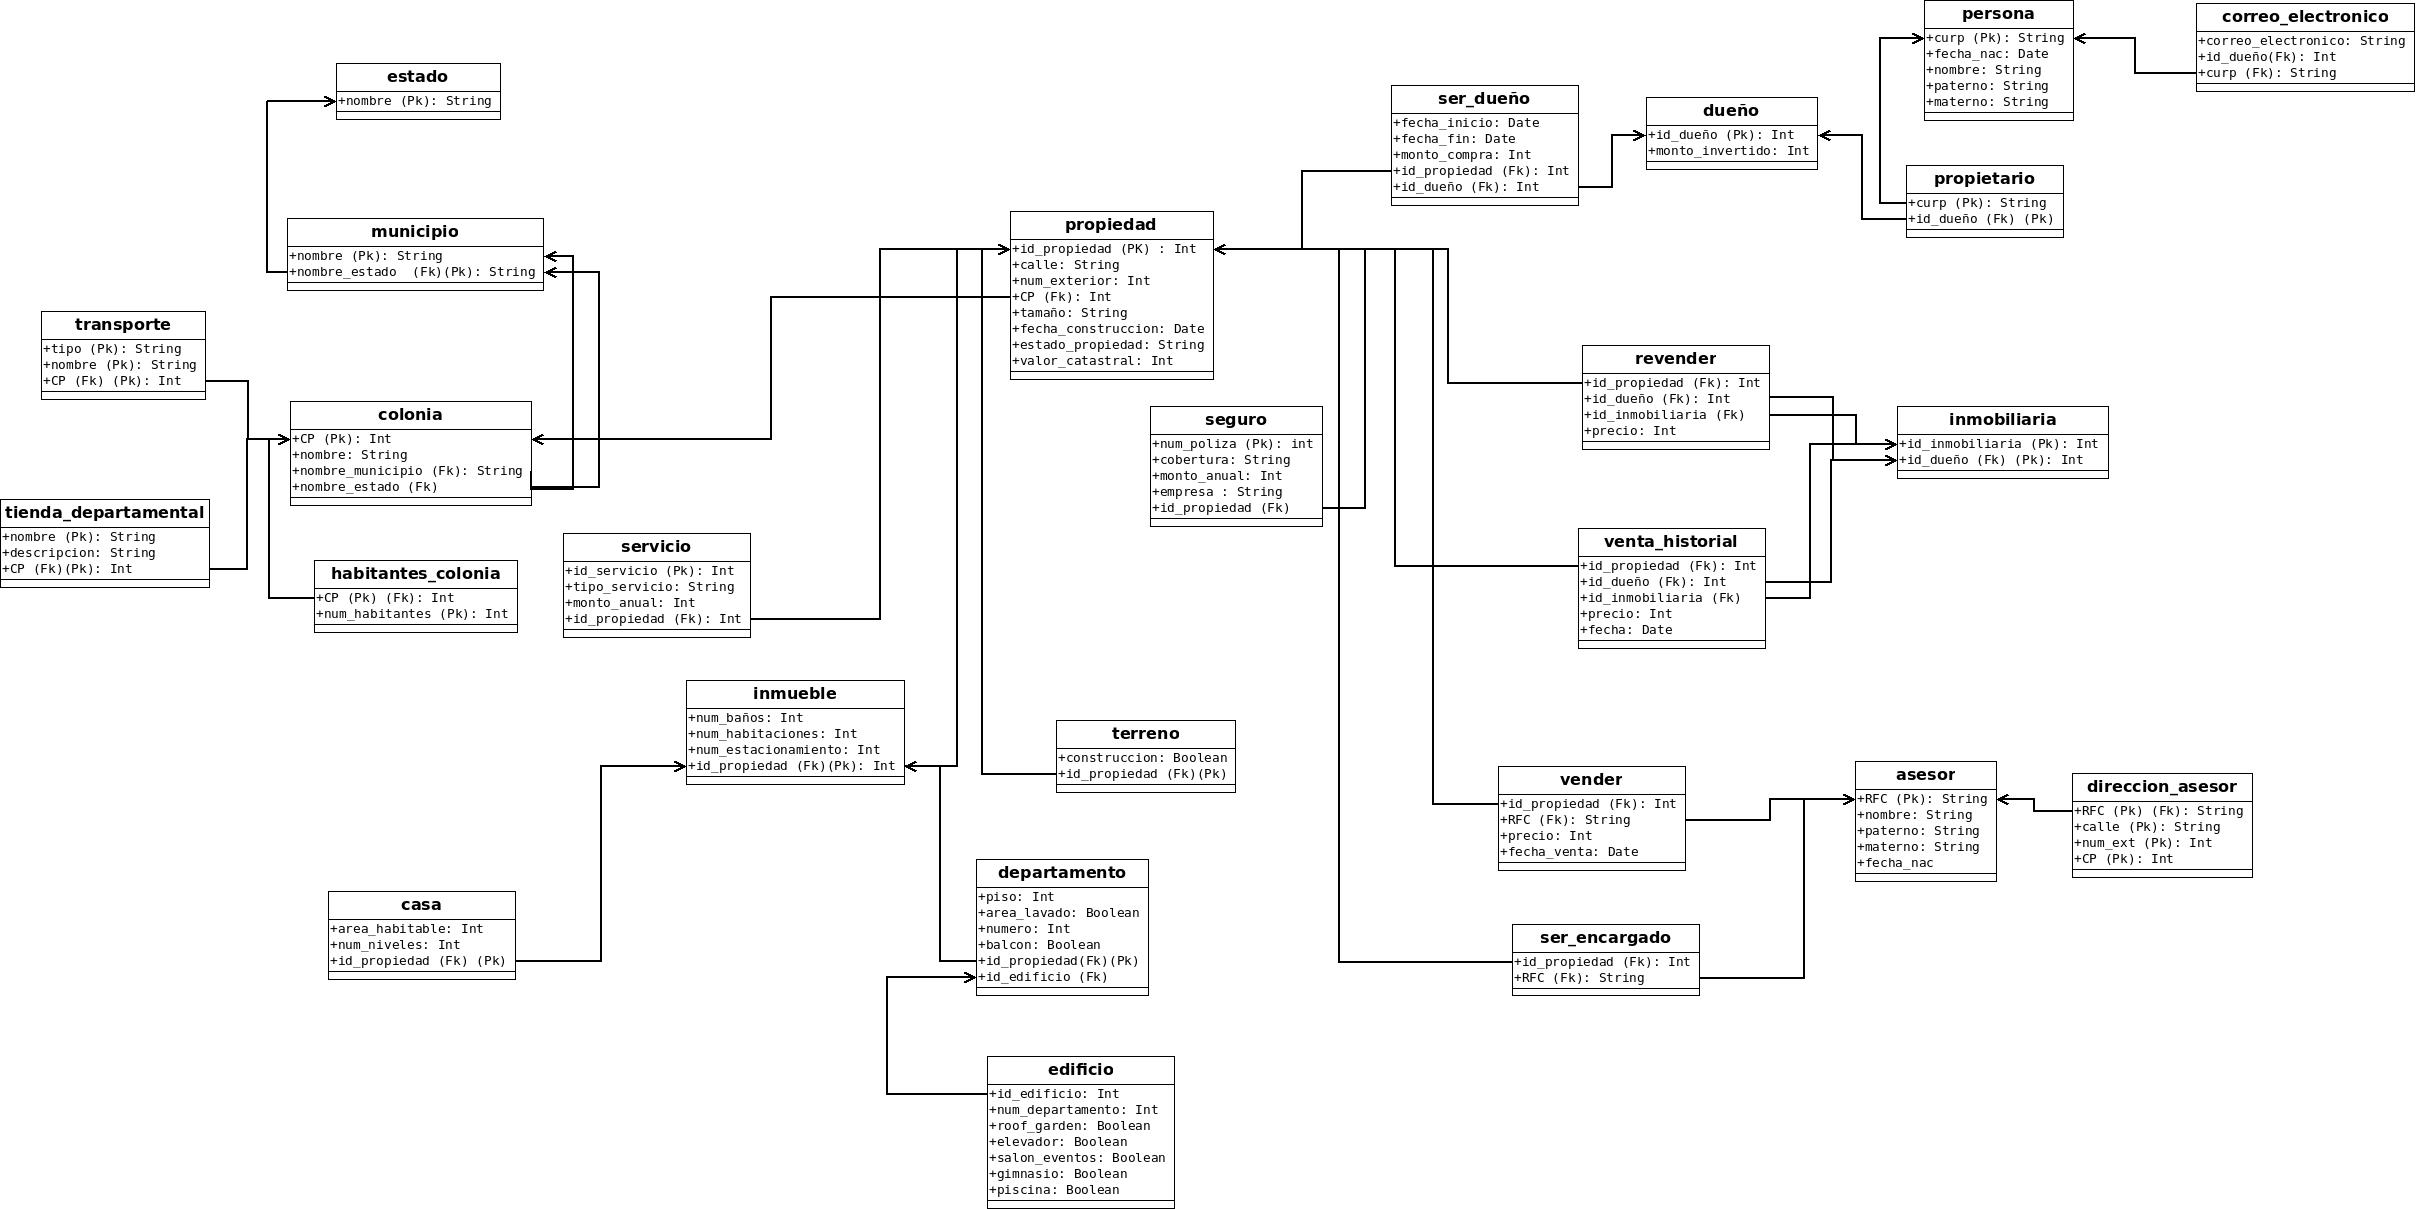
\includegraphics[width=1 \textwidth]{./modeloNormalizadoF.jpeg}
    		\caption{Esquema que corresponde a la normalización del esquema de la figura \ref{MR} usando normalización de BCNF.}
    	\end{figure}
    \end{center}
    
\end{document}	
	
	
	
	
	
	
	
	